
\documentclass[12pt]{book}

\usepackage[utf8]{inputenc}
\usepackage[greek, english]{babel}

% Packages
\usepackage{alphabeta}
\usepackage{amsmath}
\usepackage{amsthm}
\usepackage{caption}
\usepackage{color}
\usepackage{fullpage}
\usepackage{graphicx}
\usepackage{latexsym}
\usepackage{listings}
\usepackage{pxfonts}
\usepackage{stackrel}
\usepackage{titlesec}
\usepackage{subfig}
\usepackage{tikz}
\usepackage{float}
\usepackage{hyperref}
\usepackage{setspace}
\usepackage{hyperref}
\usepackage{tcolorbox}
\tcbuselibrary{theorems}

\newtcbtheorem[number within=section]{mytheorem}{Ορισμός}%
{colback=black!5,colframe=black!15!black,fonttitle=\bfseries}{th}

\newtcbtheorem[number within=section]{theorem}{Θεώρημα}%
{colback=black!5,colframe=black!15!black,fonttitle=\bfseries}{th}

% Commands
\newcommand{\N}{\mathbb{N}}
\newcommand{\R}{\mathbb{R}}
\newcommand{\code}[2]{\lstinputlisting[caption={#2}]{#1}}
\newcommand{\margin}{\hspace{4pt}}
\newcommand{\norm}[1]{\left\lVert#1\right\rVert}
\newcommand{\abs}[1]{\left\lvert#1\right\rvert}

% Environments
\newenvironment{matlab}
	{\begin{figure}[hp]\centering\captionsetup{justification=centering}}
	{\end{figure}}

\newenvironment{rcases}
	{\left.\begin{aligned}}
	{\end{aligned}\right\rbrace}

% Python Syntax Highlighting
\definecolor{string_color}{RGB}{0, 161, 13}
\definecolor{comment_color}{RGB}{46, 46, 46}
\definecolor{keyword_color}{RGB}{0, 112, 191}
\definecolor{background_color}{RGB}{250, 250, 250}

\lstset{
    framesep=15pt,
    xleftmargin=15pt,
    xrightmargin=15pt,
    language=Python,
    captionpos=b,
    numbers=right,
    numberstyle=\small\ttfamily,
    frame=lines,
    showspaces=false,
    showtabs=false,
    breaklines=true,
    showstringspaces=false,
    breakatwhitespace=true,
    commentstyle=\color{comment_color}\textit,
    keywordstyle=\bfseries\color{keyword_color}\textbf,
    stringstyle=\color{string_color}\textit,
    morekeywords={self, lambda, __init__, __del__, __name__, for, in, not, and, or, :},
    basicstyle=\small\ttfamily,
    tabsize=4,
    keepspaces=true,
    columns=flexible,
    backgroundcolor=\color{background_color}
}

% Links
\hypersetup{
    colorlinks=true,
    linkcolor=blue,
    filecolor=magenta,
    urlcolor=cyan,
}

% Lengths
\setlength{\parindent}{0in}
\setlength{\oddsidemargin}{0in}
\setlength{\textwidth}{6.5in}
\setlength{\textheight}{10in}
\setlength{\topmargin}{-1.0in}
\setlength{\headheight}{18pt}
\setlength{\parskip}{0.3cm}
\setlength{\parindent}{5ex}
\doublespacing

\theoremstyle{definition}
\newtheorem{definition}{Definition}[section]

\titlespacing*{\subsection}
{0pt}{5.5ex plus 1ex minus .2ex}{4.3ex plus .2ex}

\title{\huge Sudoku}
\author{Σιώρος Βασίλειος\\Ανδρινοπούλου Χριστίνα}
\date{Ιανουάριος 2020}

\begin{document}

\maketitle

\pagenumbering{gobble}
\pagebreak

\tableofcontents

\chapter{Abstract}

Το SUDOKU είναι ένα ιδιαίτερα δημοφιλές παιχνίδι, το οποίο έχει φανατικούς παίκτες σε όλον τον κόσμο, ανεξάρτητα ηλικιακής ομάδας, κοινωνικής τάξης ή άλλων χαρακτηριστικών. Πρόκειται για ένα παζλ βασιμένο στη λογική. \par

Στόχος του παιχνιδιού αυτού είναι ο παίκτης να συμπληρώσει τα
κενά κελιά ενός ημιτελώς συμπληρωμένου πίνακα μεγέθους
\(n \times n\) με τους κατάλληλους ακεραίους που ανήκουν στο διάστημα \(\left[1,\dots,n \right]\), με τέτοιον τρόπο ώστε κάθε γραμμή, κάθε στήλη και κάθε υποπίνακας μεγέθους \(m \times m\) να περιέχει όλους τους ακεραίους του διαστήματος  \(\left[1,\dots,n \right]\) ακριβώς μία φορά τον καθέναν. \par

Η πιο συνηθισμένη εκδοχή του SUDOKU είναι παζλ με πίνακα μεγέθους \(\left[9 \times 9\right]\) (ένα τέτοιο παράδειγμα παρατίθενται στο Figure 1.1), ωστόσο υπάρχουν και άλλες παραλλάγες του κλασσικού \(\left[9 \times 9\right] \) SUDOKU οι οποίες προκύπτουν με παραμετροποίηση του κλασσικού προτύπου SUDOKU, αλλά και προσθήκη επιπλέον περιορισμών που κάνουν την επίλυση του παζλ ακόμα πιο ενδιαφέρουσα. Σε αυτές θα αναφερθούμε εκτενώς στη συνέχεια. \par

Καθώς ο στόχος του παιχνιδιού δεν είναι μαθηματικής φύσης, η συμπλήρωση αριθμών στα κενά κελιά είναι καθαρά συμβολική. Οι αριθμοί μπορούν πολύ εύκολα να αντικατασταθούν με οποιαδήποτε ομάδα συμβόλων επιθυμεί κανείς, χωρίς να προκαλέσουν καμμία επίπτωση στην επίλυση, στη δημιουργία ή στη μαθηματική μοντελοποίηση του παζλ. Ήδη υπάρχουν διαθέσιμα SUDOKU παζλ με βάση κινέζικα σύμβολα, κινέζικους αριθμούς και σύμβολα που αναπαριστούν μερίδες σούσι. Φυσικά, αυτές οι παραλλαγές είναι ανεξάντλητες και ταυτόχρονα μηδαμινής σημασίας, γι'αυτό και δε θα επεκταθούμε περισσότερο σε αυτές. 

\begin{figure}[h]
	\centering	
	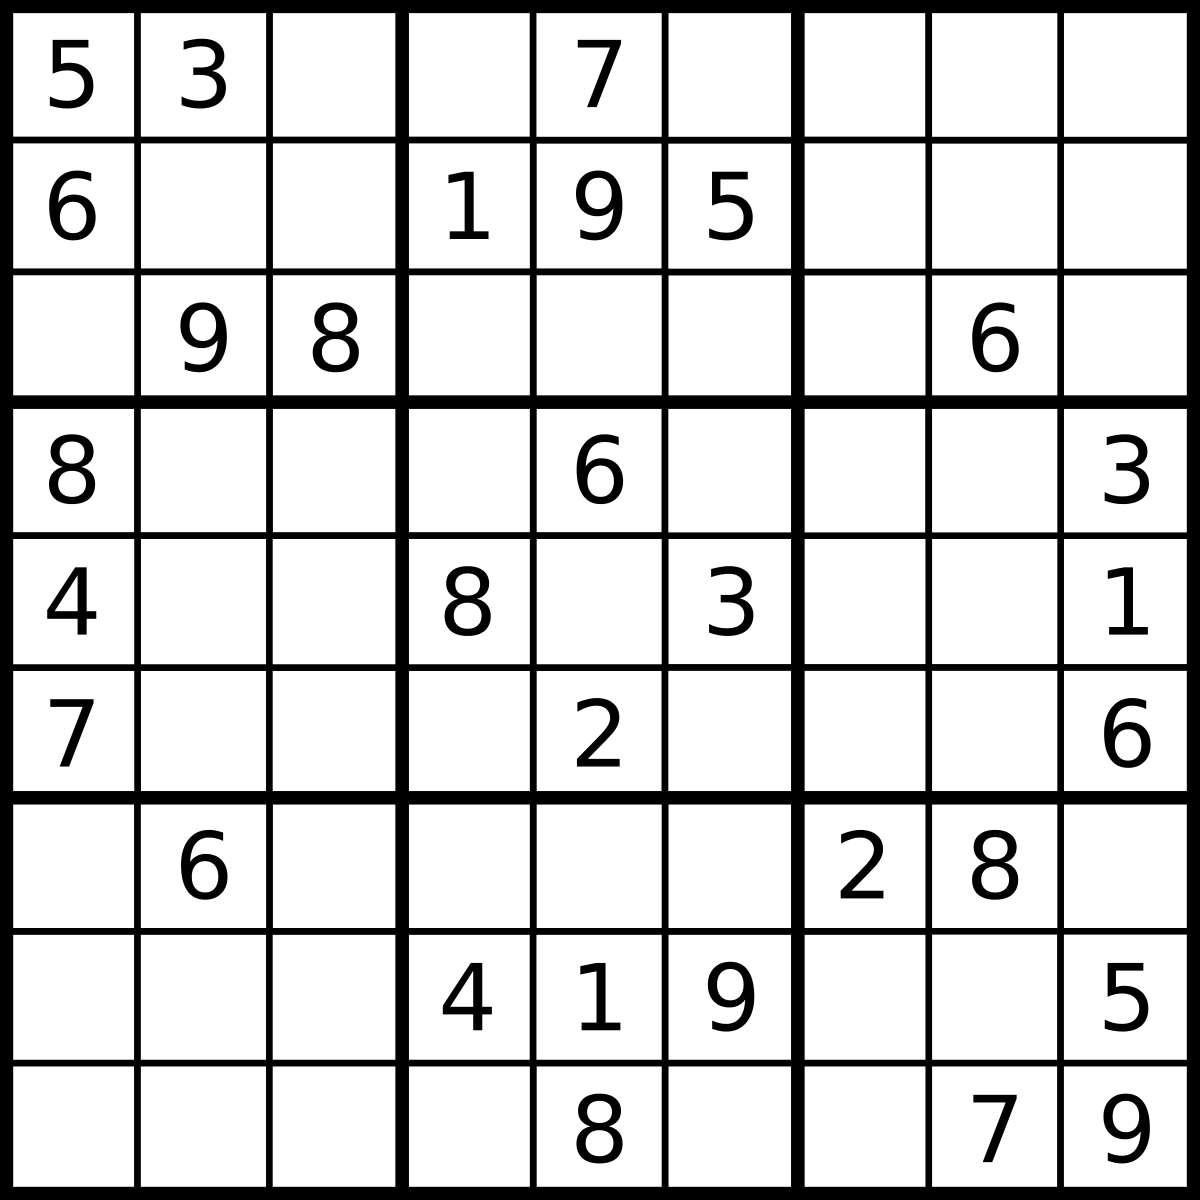
\includegraphics[scale=0.2]{Figures/classicSUDOKU.jpeg}
	\caption{Παράδειγμα κλασσικού SUDOKU \( 9 \times 9\) }
\end{figure}

\chapter{Ιστορικά στοιχεία}

Το SUDOKU, στη μορφή που το γνωρίζουμε, δημιουργήθηκε το 1979 από τον Αμερικανό αρχιτέκτονα Howard Garns (Figure 2.1). O Howard Garns \cite{1} γεννιέται τον Μάρτιο του 1905 στο Connersville του Indiana. Το 1922 αποφοιτεί από το Indianapolis Technical High School και τέσσερα χρόνια μετά αποκτά Bachelor στο Science in architectural engineering. Πεθαίνει από καρκίνο τον Οκτώβρη του 1989.  \par

\begin{figure}[h]
	\centering	
	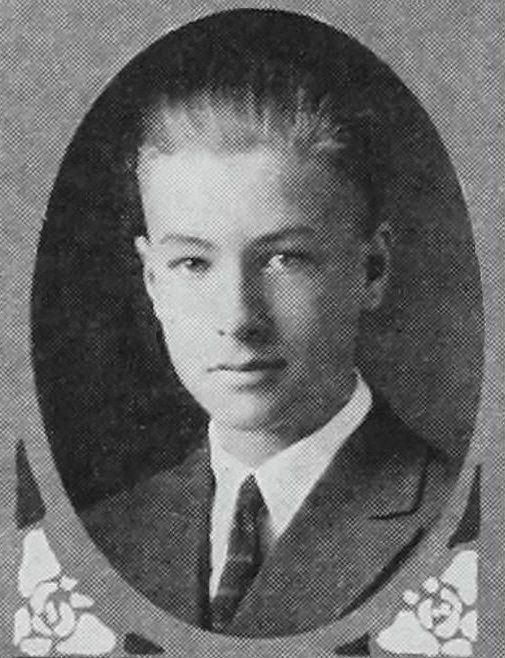
\includegraphics[scale=0.3]{Figures/Howard Garns.jpeg}
	\caption{ο Howard Garns υπήρξε ο δημιουργός του SUDOKU το 1979}
\end{figure}

Το παιχνίδι αρχικά ονομάστηκε “Number Place”, καθώς απαιτούσε την τοποθέτηση αριθμών στα κενά κελιά ενός πίνακα και
δημοσιεύτηκε στο περιοδικό Dell Pencil Puzzles and Word
Games το 1979. \par

Ενα χρόνο μετά το παιχνίδι έγινε ιδιαίτερα δημοφιλές στην Ιαπωνία και μετονομάστηκε σε “suji wa dokushin ni
kagiru”(SUDOKU), που σημαίνει ότι "τα ψηφία είναι περιορισμένα σε κάποιο κανόνα". \par

Το SUDOKU έγινε ιδιαίτερα αγαπητό στην Ιαπωνία, με τις μηνιαίες πωλήσεις SUDOKU περιοδικών να ανέρχονται στα
600.000 αντίτυπα κάθε μήνα.
Οι Ιάπωνες υιοθέτησαν το SUDOKU ως συνήθεια για δύο
βασικούς λόγους. Ο πρώτος λόγος έχει να κάνει με τη γλώσσα τους. Η γλώσσα τους δεν ήταν κατάλληλη, όπως άλλες γλώσσες σαν την ελληνική, για την ανάπτυξη σταυρόλεξων, οπότε υστερούσαν σε τέτοιου είδους παιχνίδια. Ο δεύτερος λόγος σχετίζεται με τις συνήθειες των κατοίκων της Ιαπωνίας, οι οποίοι συνηθίζουν να μετακινούνται σε καθημερινή βάση με τρένα και λεωφορεία και με αυτόν τον τρόπο διανύουν μεγάλες αποστάσεις και περνούν πολύ από τον χρόνο τους σε καθημερινή βάση μέσα σε μέσα μαζικής μεταφοράς. Συνεπώς, η ύπαρξη ενός τέτοιου παιχνιδιού έκανε τις χρονοβώρες μετακινήσεις τους πιο ευχάριστες και επικοδομητικές. \par 

\begin{figure}[h]
	\centering	
	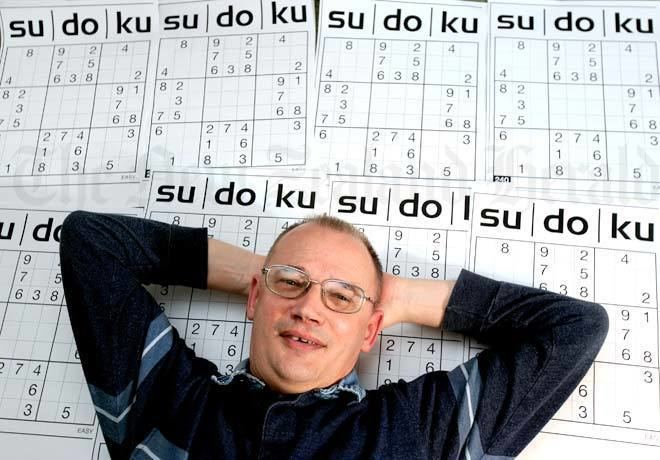
\includegraphics[scale=0.45]{Figures/WayneGould.jpg}
	\caption{ο Wayne Gould έκανε και πάλι αγαπητό το SUDOKU στη Δύση}
\end{figure}

Ο άνθρωπος που έφερε πίσω στον Δυτικό κόσμο το SUDOKU ήταν ο Wayne Gould (Figure 2.2). Ο Νεοζηλανδός Wayne Gould γεννήθηκε στις 3 Ιουλίου 1945 και υπήρξε δικαστής. Ωστόσο, εκείνο που τον έκανε ιδιαίτερα διάσημο δεν ήταν οι δικαστικές του ικανότητες, αλλά το γεγονός ότι έκανε το SUDOKU γνωστό στον Δυτικό κόσμο. Το 1997 βρισκόταν στο Τόκιο και ανακάλυψε ενα SUDOKU σε κάποιο βιβλιοπωλείο. Η ιδέα αυτού του παιχνιδιού τον ενθουσίασε ιδιαιτέρως. Μερικά χρόνια αργότερα έφτιαξε το πρωτο πρόγραμμα που δημιουργούσε SUDOKU παζλ διαφορετικών επιπέδων δυσκολίας. Ο Wayne Gould καταφέρνει τον Νοέμβριο του 2004 να πείσει το "The Times" στον Λονδίνο να δημοσιεύσουν ένα παζλ SUDOKU. Έπειτα από εκείνη τη δημοσίευση, ο κόσμος αγκάλιασε το παιχνίδι αυτό και για πολλούς ανθρώπους ανά τον κόσμο έγινε αγαπημένη συνήθεια.

\chapter{Εισαγωγή}

Το SUDOKU είναι ένα παζλ βασιμένο στη λογική. Στόχος του παιχνιδιού αυτού είναι η συμπλήρωση των
κενών κελιών ενός ημιτελώς συμπληρωμένου πίνακα μεγέθους
\(n \times n\) με τους κατάλληλους ακεραίους που ανήκουν στο διάστημα \(\left[1,\dots,n \right]\), με τέτοιον τρόπο ώστε κάθε γραμμή, κάθε στήλη και κάθε υποπίνακας μεγέθους \(m \times m\), όπου \(m = \sqrt{n} \) και \( m \ge 0\), να περιέχει όλους τους ακεραίους του διαστήματος  \(\left[1,\dots,n \right]\) ακριβώς μία φορά τον καθέναν. \par

\begin{mytheorem}{SUDOKU}{}
	Οι κανόνες για το κλασσικό SUDOKU σε έναν πίνακα μεγέθους \(n \times n\) με υποπίνακες μεγέθους \(m \times m\), 	όπου \(m = \sqrt{n}\) είναι: \\
	\(\bullet\) Κάθε γραμμή του πίνακα μεγέθους n να περιέχει ακριβώς μια φορά κάθε ακέραιο αριθμό από το 1 ως το n. \\
	\(\bullet\) Κάθε στήλη του πίνακα μεγέθους n να περιέχει ακριβώς μια φορά κάθε ακέραιο αριθμό από το 1 ως το n. \\
	\(\bullet\) Κάθε υποπίνακας μεγέθους \(m \times m\) να περιέχει ακριβώς μια φορά κάθε ακέραιο αριθμό από το 1 ως το n. \\
\end{mytheorem}

Το επίπεδο δυσκολίας από παζλ σε παζλ διαφέρει και σχετίζεται με την ποσότητα των συμπληρωμένων κελιών, αλλά και με τη θέση τους μέσα στο παζλ. \par

Η μελέτη μας θα εστιάσει στις μαθηματικές μεθοδολογίες για την επίλυση SUDOKU παζλ και στις μαθηματικές τεχνικές για τη δημιουργία SUDOKU παζλ. \par 

Κατά την παρουσίαση των μαθηματικών μεθοδολογιων που επιλύουν παζλ SUDOKU θα παρουσιάσουμε τη μοντελοποίηση του προβλήματος της επίλυσης του παζλ ως
πρόβλημα γραμμικού προγραμματισμού, έπειτα την επαλήθευση με χρήση MATLAB που έχει γίνει και τέλος θα αναφερθούμε σε ενδιαφέρουσες παραλλαγές του κλασσικού SUDOKU. \par

Στο κεφάλαιο που αφορά τις μαθηματικές τεχνικές για τη δημιουργία παζλ SUDOKU θα μελετήσουμε αρχικά την κατασκευή SUDOKU με bruteforce κι έπειτα θα εστιάσουμε στην κατασκευή SUDOKU με βάση παλαιότερα παζλ. \par

\chapter{Επίλυση SUDOKU παζλ}
\section{Μαθηματική μοντελοποίηση}

Στο κεφάλαιο αυτό θα παρουσιάσουμε μία μαθηματική μοντελοποίηση του προβλήματος της επίλυσης των παζλ SUDOKU. Σκοπός του παρόντος κεφαλαίου είναι να προτείνουμε μια μαθηματική μοντελοποίηση που θα καθιστά δυνατή την εύρεση της λύσης του παζλ, αν υπάρχει, από έναν μαθηματικό αλγόριθμο. \par 

Θεωρούμε το πρόβλημα της επίλυσης ενός \(n \times n\) παζλ SUDOKU ως πρόβλημα δυαδικού (;) γραμμικού προγραμματισμού. Ο δυαδικός γραμμικός προγραμματισμός είναι ένος τρόπος επίλυσης ενός συστήματος γραμμικών ανισοτήτων με δυαδικούς αγνώστους \cite{2}. \par

Έστω, ο \(n \times n\) πίνακας SUDOKU και οι υποπίνακες του μεγέθους \(m \times m\). Ορίζουμε τις μεταβλητές απόφασης ως εξής: \\

\[
  		x_{ijk} = 
  		\begin{cases}
  			1 &\quad\text{αν το κελι (i,j) του πίνακα περιέχει τον ακέραιο k}\\
	  		0 &\quad\text{αλλιώς} \\
 
  		\end{cases}
\]

Η μοντελοποίηση του προβλήματος σύμφωνα με το \cite{3} δίνεται παρακάτω:

\begin{align*}
	\min \quad 0^{T}x \\
	\begin{aligned}
		\textup{s.t.}\quad
			\sum_{i=1}^{n}x_{ijk} = 1 &\quad j=1:n, \quad k=1:n \quad \text{μόνο ένα k σε κάθε στήλη του πίνακα} \\
			\sum_{j=1}^{n}x_{ijk} = 1 &\quad i=1:n, \quad k=1:n \quad \text{μόνο ένα k σε κάθε γραμμή του πίνακα} \\
			\sum_{j=mq-m+1}^{mq} {\sum_{i=mp-m+1}^{mp}x_{ijk}} = 1 &\quad k=1:n, \quad p=1:m, \quad q=1:m \quad \text{μόνο ένας ακέραιος k σε κάθε υποπίνακα} \\
			\sum_{k=1}^{n}x_{ijk} = 1 &\quad i=1:n, \quad j=1:n \quad \text{όλα τα κελιά του πίνακα πρέπει να συμπληρωθούν} \\
			x_{ijk} = 1 \forall (i,j,k) \in G &\quad \text{τα κελιά του πίνακα που είναι συμπληρωμένα είναι "on"} \\
			x_{ijk} \in {0,1}&
	\end{aligned}
\end{align*}

Ουσιαστικά το πρόβλημα επίλυσης ενός SUDOKU παζλ είναι πρόβλημα ικανοποίησης περιορισμών. \par 

Ένα πρόβλημα ικανοποίησης περιορισμών ορίζεται από δύο σύνολα: το σύνολο μεταβλητών, \(X_1, X_2, \dots, X_t\), και το σύνολο περιορισμών, \(C_1, C_2, \dots, C_z\). Κάθε μεταβλητή \(X_i\) με \(1 \leq i \leq t\) λαμβάνει τιμές από ένα πεδίο \(D_i\). Κάθε περιορισμός \(C_j\) με \(1 \leq j \leq z\) αφορά κάποιο υποσύνολο των μεταβλητών και καθορίζει ποιος είναι ο επιτρεπτός συνδυασμός τιμών για αυτό το υποσύνολο μεταβλητών. Μία ανάθεση τιμών που δεν παραβιάζει κανέναν περιορισμό του προβλήματος ονομάζεται συνεπής ή νόμιμη ανάθεση, ενώ μία ανάθεση που αποδίδει τιμές σε όλες τις μεταβλητές ονομάζεται πλήρης. Αν μια ανάθεση είναι συνεπής και πλήρης, τότε καλείται λύση του προβλήματος. Να σημειωθεί ότι στα προβλήματα ικανοποίησης περιορισμών η διατύπωση αντικειμενικής συνάρτησης δεν είναι υποχρεωτική \cite{4}. \par

Στόχος μας είναι να ανακαλύψουμε μία πλήρη και συνεπή ανάθεση στο πρόβλημα που μοντελοποιήσαμε προηγουμένως. Η ύπαρξη αντικειμενικής συνάρτησης στη μοντελοποίηση μας δεν είναι κομβικής σημασίας, ωστόσο η χρήση της θα φανεί στη συνέχεια.

\section{Επαλήθευση της μαθηματικής μοντελοποίησης}

\subsection{Επαλήθευση με Matlab}

Η επαλήθευση της ορθότητας της παραπάνω μοντελοποίησης μπορεί να γίνει με Matlab. Όπως προτείνεται στο \cite{3} το πρόγραμμα sudoku.m, το οποίο μπορεί κανείς να το βρει στο \url{http://aristotle.davidson.edu/chartier/sudoku/sudoku.m} βρίσκει λύση στο πρόβλημα επίλυσης ενός παζλ SUDOKU. \par

Το πρόγραμμα λαμβάνει ως είσοδο τα κελιά του πίνακα που είναι ήδη συμπληρωμένα κι έπειτα με κλήση της συνάρτησης bintprog που είναι υλοποιημένη στο Matlab λύνει το SUDOKU σε μερικά δευτερόλεπτα. 

\subsection{Επαλήθευση με Python}
.......

\section{Μαθηματική μοντελοποίηση παραλλαγμένων SUDOKU παζλ}

Στο κεφάλαιο αυτό θα αναφερθούμε σε ορισμένες παραλλαγές του κλασσικού παζλ SUDOKU, που καθιστούν την επίλυσή τους πιο απαιτητική σε σχέση με το κλασσικό παζλ, για τους παίκτες SUDOKU. Ωστόσο, αυτή η δυσκολία δεν αντικατοπτρίζεται και στη μοντελοποίηση τους. \par 

Θα δούμε στη συνέχεια ότι η μοντελοποίηση των παραλλαγμένων παζλ SUDOKU δε διαφέρει ιδιαίτερα από τη μοντελοποίηση για τα κλασσικά παζλ SUDOKU. Το μόνο που αλλάζει εδώ είναι ότι προκύπτει η ανάγκη για την προσθήκη μερικών νέων περιορισμών, ανάλογα με την παραλλαγή του παζλ κάθε φορα. \par

Όλα τα παραπάνω θα γίνουν σαφώς πιο κατανοητά στη συνέχεια αυτού του κεφαλαίου, καθώς θα μελετάμε τις διάφορες διάσημες παραλλαγές του κλασσικού SUDOKU. Θα προτείνουμε τρόπους μοντελοποίησης όλων των παραλλαγών, άρα και τρόπους λύσης, όπως αυτοί προέκυψαν από το \cite{3}.

\subsection{SUDOKU X}

Το SUDOKU X είναι μία παραλλαγή του κλασσικού SUDOKU. Η επίλυση ενός τέτοιου παζλ είναι η ίδια με εκείνη ενός κλασσικού SUDOKU με τον επιπλεόν κανόνα ότι οι δύο μεγάλες διαγώνιοι του πίνακα πρέπει να περιέχουν κάθε ψηφίο από το 1 μέχρι το n ακριβώς μία φορά η κάθε μία. Παραθέτουμε ένα παράδειγμα SUDOKU X μεγέθους \(9 \times 9 \) στο Figure 4.1.\par

\begin{mytheorem}{SUDOKU}{}
	Οι κανόνες για το SUDOKU X σε έναν πίνακα μεγέθους \(n \times n\) με υποπίνακες μεγέθους \(m \times m\), 	όπου \(m = \sqrt{n}\) είναι: \\
	\(\bullet\) Κάθε γραμμή του πίνακα μεγέθους n να περιέχει ακριβώς μια φορά κάθε ακέραιο αριθμό από το 1 ως το n. \\
	\(\bullet\) Κάθε στήλη του πίνακα μεγέθους n να περιέχει ακριβώς μια φορά κάθε ακέραιο αριθμό από το 1 ως το n. \\
	\(\bullet\) Κάθε υποπίνακας μεγέθους \(m \times m\) να περιέχει ακριβώς μια φορά κάθε ακέραιο αριθμό από το 1 ως το n. \\
	\(\bullet\) Η διαγώνιος του πίνακα που ξεκινά από το κελί (1,1) και καταλήγει στο κελί (n,n) να περιέχει ακριβώς μια φορά κάθε ακέραιο αριθμό από το 1 ως το n. \\
	\(\bullet\) Η διαγώνιος του πίνακα που ξεκινά από το κελί (1,n) και καταλήγει στο κελί (n,1) να περιέχει ακριβώς μια φορά κάθε ακέραιο αριθμό από το 1 ως το n. \\

\end{mytheorem}

Προφανώς, κάθε λύση για ένα συγκεκριμένο SUDOKU X παζλ είναι λύση και για το αντίστοιχο κλασσικό παζλ, το αντίθετο όμως δεν ισχυεί πάντα. \par

\begin{figure}[h]
	\centering	
	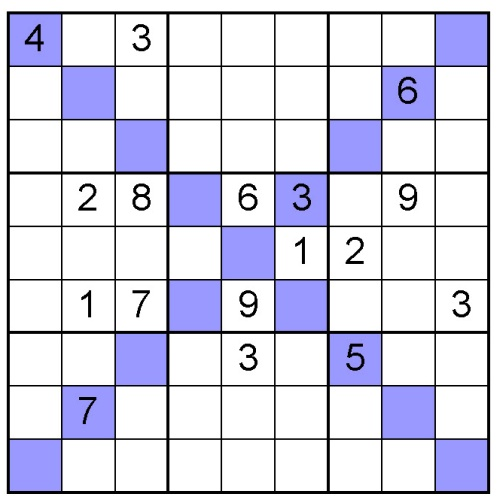
\includegraphics[scale=1.5]{Figures/sudokuX.jpg}
	\caption{Παράδειγμα ενός SUDOKU X παζλ. Οι δύο μεγάλες διαγώνιοι είναι σημειωμένες με μωβ χρώμα. Η κάθε μία πρέπει να περιέχει όλους τους αριθμούς από το 1 εως και το 9 ακριβώς μία φορα τον καθέναν.}
\end{figure}

Η μαθηματική μοντελοποίηση αυτής της παραλλαγής απαιτεί την προσθήκη επιπλέον περιορισμών που αντανακλούν τον επιπρόσθετο κανόνα που προαναφέραμε. Η μοντελοποίηση είναι όπως ορίστηκε στο κεφάλαιο 4.1 με την εξής προσθήκη στους περιορισμούς: \\

Για τη μία διαγώνιο του πίνακα:

\begin{align*}
	\sum_{r=1}^{n} x_{rrk} = 1 \quad k=1:9 \quad \text{μόνο ένα k στη διαγώνιο που ξεκινά από το κελι (1,1) και καταλήγει στο κελι (n,n)}
\end{align*}

και για την άλλη διαγώνιο του πίνακα:

\begin{align*}
\sum_{r=1}^{n} x_{r(n+1-r)k} = 1 \quad k=1:9 \quad \text{μόνο ένα k στη διαγώνιο που ξεκινά από το κελι (1,n) και καταλήγει στο κελι (n,1)}
\end{align*}

Συνεπώς, η τελική μαθηματική μοντελοποίηση για το SUDOKU X είναι:

\begin{align*}
	\begin{aligned}
		\min &\quad 0^{T}x \\
		\textup{s.t.}\quad
		\sum_{i=1}^{n}x_{ijk} = 1 &\quad j=1:n, \quad k=1:n \quad \text{μόνο ένα k σε κάθε στήλη του πίνακα} \\
		\sum_{j=1}^{n}x_{ijk} = 1 &\quad i=1:n, \quad k=1:n \quad \text{μόνο ένα k σε κάθε γραμμή του πίνακα} \\
		\sum_{j=mq-m+1}^{mq} {\sum_{i=mp-m+1}^{mp}x_{ijk}} = 1 &\quad k=1:n, \quad p=1:m, \quad q=1:m \quad \text{μόνο ένας ακέραιος k σε κάθε υποπίνακα} \\
		\sum_{k=1}^{n}x_{ijk} = 1 &\quad i=1:n, \quad j=1:n \quad \text{όλα τα κελιά του πίνακα πρέπει να συμπληρωθούν} \\
		\sum_{r=1}^{n} x_{rrk} = 1 &\quad k=1:9 \quad \text{μόνο ένα k στη διαγώνιο που ξεκινά από το κελι (1,1) και καταλήγει στο κελι (n,n)} \\
		\sum_{r=1}^{n} x_{r(n+1-r)k} = 1 &\quad k=1:9 \quad \text{μόνο ένα k στη διαγώνιο που ξεκινά από το κελι (1,n) και καταλήγει στο κελι (n,1)} \\
		x_{ijk} = 1 \forall (i,j,k) \in G &\quad \text{τα κελιά του πίνακα που είναι συμπληρωμένα είναι "on"} \\
		x_{ijk} \in {0,1}&
\end{aligned}
\end{align*}

\subsection{Four Square SUDOKU}

Το Four Square SUDOKU περιέχει τους κανόνες του κλασσικού SUDOKU και έναν επιπλέον κανόνα. Αν υποθέσουμε ότι αναφερόμαστε σε \(9 \times 9\) πίνακα, τότε στο Four Square SUDOKU δημιουργόυμε τέσσερις επιπλέον υποπεριοχές στον πίνακα μεγέθους \(3 \times 3\), όπως φαίνεται στο Figure 4.2. Στίς περιοχές αυτες πρέπει να περιέχονται όλοι οι ακέραιοι αριθμοί από το 1 ως το 9. \par 

\begin{mytheorem}{Four Square SUDOKU}{}
	Οι κανόνες για το Four Square SUDOKU σε έναν πίνακα μεγέθους \(9 \times 9\) με υποπίνακες μεγέθους \(3 \times 3\) είναι: \\
	\(\bullet\) Κάθε γραμμή του πίνακα μεγέθους 9 να περιέχει ακριβώς μια φορά κάθε ακέραιο αριθμό από το 1 ως το n. \\
	\(\bullet\) Κάθε στήλη του πίνακα μεγέθους 9 να περιέχει ακριβώς μια φορά κάθε ακέραιο αριθμό από το 1 ως το 9. \\
	\(\bullet\) Κάθε υποπίνακας μεγέθους \(3 \times 3\) να περιέχει ακριβώς μια φορά κάθε ακέραιο αριθμό από το 1 ως το 9. \\
	\(\bullet\) Κάθε υποπεριοχή μεγέθους
\(3 \times 3\) να περιέχει όλους τους ακέραιους από το 1 ως το 9. \\
\end{mytheorem}

\begin{figure}[h]
	\centering	
	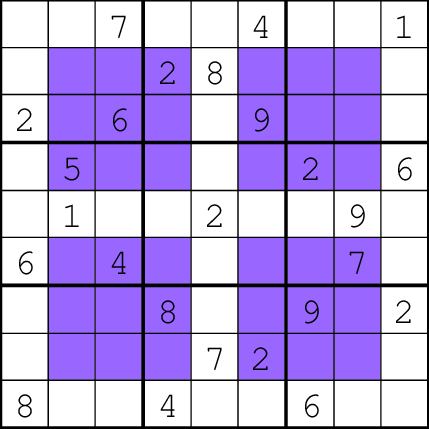
\includegraphics[scale=0.7]{Figures/An-example-Four-Square-Sudoku-puzzle.png}
	\caption{Παράδειγμα ενός Four Square SUDOKU παζλ. Οι τέσσερις περιοχές είναι σημειωμένες με μωβ χρώμα. Η κάθε μία πρέπει να περιέχει όλους τους αριθμούς από το 1 εως και το 9 ακριβώς μία φορα τον καθέναν.}
\end{figure}

Η μοντελοποίηση της συγκεκριμένης παραλλαγής SUDOKU απαιτεί την προσθήκη επιπλέον περιορισμών, που αποτυπώνουν τον τελευταίο κανόνα του Ορισμού 4.3.2. Οι επιλογές για τα i και j καθορίζουν τις υποπεριοχές. Οι περιορισμοί που δίνουμε στη συνέχεια αποτυπώνουν τις μωβ υποπεριοχές του Figure 4.2.\\

\begin{align*}
	\sum_{r=i}^{i+2}{\sum_{c=j}^{j+2}x_{rck}} = 1 \quad i=2,6; \quad j=2,6; \quad k=1:9
\end{align*}

Συνεπώς, η τελική μαθηματική μοντελοποίηση για το Four Square SUDOKU είναι:

\begin{align*}
	\begin{aligned}
		\min &\quad 0^{T}x \\
		\textup{s.t.}\quad
		\sum_{i=1}^{9}x_{ijk} = 1 &\quad j=1:9, \quad k=1:9 \quad \text{μόνο ένα k σε κάθε στήλη του πίνακα} \\
		\sum_{j=1}^{9}x_{ijk} = 1 &\quad i=1:9, \quad k=1:9 \quad \text{μόνο ένα k σε κάθε γραμμή του πίνακα} \\
		\sum_{j=3q-3+1}^{3q} {\sum_{i=3p-3+1}^{3p}x_{ijk}} = 1 &\quad k=1:9, \quad p=1:3, \quad q=1:3 \quad \text{μόνο ένας ακέραιος k σε κάθε υποπίνακα} \\
		\sum_{k=1}^{9}x_{ijk} = 1 &\quad i=1:9, \quad j=1:9 \quad \text{όλα τα κελιά του πίνακα πρέπει να συμπληρωθούν} \\
		\sum_{r=i}^{i+2}{\sum_{c=j}^{j+2}x_{rck}} = 1 &\quad i=2,6; \quad j=2,6; \quad k=1:9 \quad \text{οι επιπλέον υποπεριοχές πρέπει να περιέχουν όλους τους ακέραιους από το 1 ως το 9 ακριβώς μία φορά} \\
		x_{ijk} = 1 \forall (i,j,k) \in G &\quad \text{τα κελιά του πίνακα που είναι συμπληρωμένα είναι "on"} \\
		x_{ijk} \in {0,1}&
	\end{aligned}
\end{align*}

\subsection{Four Pyramids SUDOKU}

Η παραλλαγή Four Pyramids SUDOKU είναι παρόμοια με την Four Square SUDOKU παραλλαγή που αναφέραμε στην προηγούμενη υποενότητα, με τη διαφορά ότι εδώ οι επιπλέον υποπεριοχές του πίνακα στις οποίες πρέπει να περιέχονται όλοι οι ακέραιοι αριθμοί από το 1 ως το 9 ακριβώς μία φορά στην κάθε μία δεν έχουν πλέον τη μορφή τετραγώνων, αλλά τριγωνική μορφή.

\begin{mytheorem}{Four Pyramids SUDOKU}{}
	Οι κανόνες για το Four Pyramids SUDOKU σε έναν πίνακα μεγέθους \(9 \times 9\) με υποπίνακες μεγέθους \(3 \times 3\) είναι: \\
	\(\bullet\) Κάθε γραμμή του πίνακα μεγέθους 9 να περιέχει ακριβώς μια φορά κάθε ακέραιο αριθμό από το 1 ως το n. \\
	\(\bullet\) Κάθε στήλη του πίνακα μεγέθους 9 να περιέχει ακριβώς μια φορά κάθε ακέραιο αριθμό από το 1 ως το 9. \\
	\(\bullet\) Κάθε υποπίνακας μεγέθους \(3 \times 3\) να περιέχει ακριβώς μια φορά κάθε ακέραιο αριθμό από το 1 ως το 9. \\
	\(\bullet\) Κάθε υποπεριοχή μεγέθους
\(3 \times 3\) να περιέχει όλους τους ακέραιους από το 1 ως το 9. \\
\end{mytheorem}

\begin{figure}[h]
	\centering	
	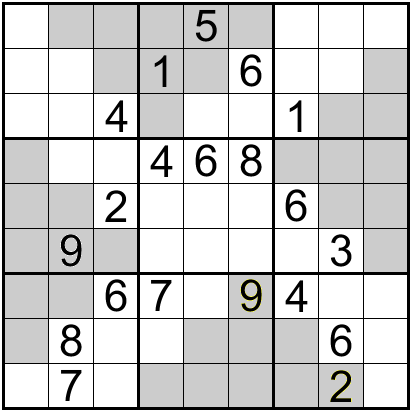
\includegraphics[scale=0.7]{Figures/Pyramid Sudoku.png}
	\caption{Παράδειγμα ενός Four Pyramids SUDOKU παζλ. Οι τέσσερις τριγωνικές περιοχές είναι σημειωμένες με γκρί χρώμα. Η κάθε μία πρέπει να περιέχει όλους τους αριθμούς από το 1 εως και το 9 ακριβώς μία φορα τον καθέναν.}
\end{figure}

Η μαθηματική μοντελοποίηση απαιτεί την προσθήκη των παρακάτων περιορισμών στη μοντελοποίηση του κλασσικού SUDOKU.

\begin{align*}
	\sum_{r=1}^{3}{\sum_{c=3+r}^{9-r} x_{rck}} = 1 \quad k=1:9 \\
	\sum_{c=1}^{3}{\sum_{r=1+c}^{7-c} x_{rck}} = 1 \quad k=1:9 \\\\
	\sum_{r=7}^{9}{\sum_{c=11-r}^{r-7} x_{rck}} = 1 \quad k=1:9 \\
	\sum_{c=7}^{9}{\sum_{r=13-c}^{c-1} x_{rck}} = 1 \quad k=1:9 \\	
\end{align*}

Οπότε, τελικά, η μαθηματική μοντελοποίηση για το Four Pyramids SUDOKU, αν απαριθμήσουμε τις πυραμίδες με τη φορά του ρολογιού, είναι:

\begin{align*}
	\begin{aligned}
		\min &\quad 0^{T}x \\
		\textup{s.t.}\quad
		\sum_{i=1}^{9}x_{ijk} = 1 &\quad j=1:9, \quad k=1:9 \quad \text{μόνο ένα k σε κάθε στήλη του πίνακα} \\
		\sum_{j=1}^{9}x_{ijk} = 1 &\quad i=1:9, \quad k=1:9 \quad \text{μόνο ένα k σε κάθε γραμμή του πίνακα} \\
		\sum_{j=3q-3+1}^{3q} {\sum_{i=3p-3+1}^{3p}x_{ijk}} = 1 &\quad k=1:9, \quad p=1:3, \quad q=1:3 \quad \text{μόνο ένας ακέραιος k σε κάθε υποπίνακα} \\
		\sum_{k=1}^{9}x_{ijk} = 1 &\quad i=1:9, \quad j=1:9 \quad \text{όλα τα κελιά του πίνακα πρέπει να συμπληρωθούν} \\
		\sum_{r=1}^{3}{\sum_{c=3+r}^{9-r} x_{rck}} = 1 &\quad k=1:9 \quad \text{η πρώτη πυραμίδα να έχει μόνο ένα k} \\
		\sum_{c=1}^{3}{\sum_{r=1+c}^{7-c} x_{rck}} = 1 &\quad k=1:9 \quad \text{η δεύτερη πυραμίδα να έχει μόνο ένα k}\\
		\sum_{r=7}^{9}{\sum_{c=11-r}^{r-7} x_{rck}} = 1 &\quad k=1:9 \quad \text{η τρίτη πυραμίδα να έχει μόνο ένα k} \\
		\sum_{c=7}^{9}{\sum_{r=13-c}^{c-1} x_{rck}} = 1 &\quad k=1:9 \quad \text{η τέταρτη πυραμίδα να έχει μόνο ένα k} \\
		x_{ijk} = 1 \forall (i,j,k) \in G &\quad \text{τα κελιά του πίνακα που είναι συμπληρωμένα είναι "on"} \\
		x_{ijk} \in {0,1}&
	\end{aligned}
\end{align*}

\subsection{Position SUDOKU}

Στην παραλλαγή Position SUDOKU εκτός από τους κανόνες του κλασσικού SUDOKU πρέπει να ικανοποιείται και ένα επιπλέον περιορισμός. Τα κελιά (1,1) σε όλους τους \(3 \times 3\) υποπίνακες πρέπει να περιέχουν όλους τους ακέραιους από το 1 ως το 9 ακριβώς μια φορά, αντίστοιχα τα κελιά (1,2) όλων των υποπινάκων κοκ. Οι κανόνες του Position SUDOKU συνοψίζονται στον παρακάτω ορισμό. \par 

\begin{mytheorem}{Position SUDOKU}{}
	Οι κανόνες για το Position SUDOKU σε έναν πίνακα μεγέθους \(9 \times 9\) με υποπίνακες μεγέθους \(3 \times 3\) είναι: \\
	\(\bullet\) Κάθε γραμμή του πίνακα μεγέθους 9 να περιέχει ακριβώς μια φορά κάθε ακέραιο αριθμό από το 1 ως το n. \\
	\(\bullet\) Κάθε στήλη του πίνακα μεγέθους 9 να περιέχει ακριβώς μια φορά κάθε ακέραιο αριθμό από το 1 ως το 9. \\
	\(\bullet\) Κάθε υποπίνακας μεγέθους \(3 \times 3\) να περιέχει ακριβώς μια φορά κάθε ακέραιο αριθμό από το 1 ως το 9. \\
	\(\bullet\) Κάθε κελί (i,j) με i=1:9 και j=1:9 σε όλους τους υποπίνακες \(3 \times 3\) να περιέχει ακριβώς μια φορά κάθε ακέραιο αριθμό από το 1 ως το 9.
\end{mytheorem}

\begin{figure}[h]
	\centering	
	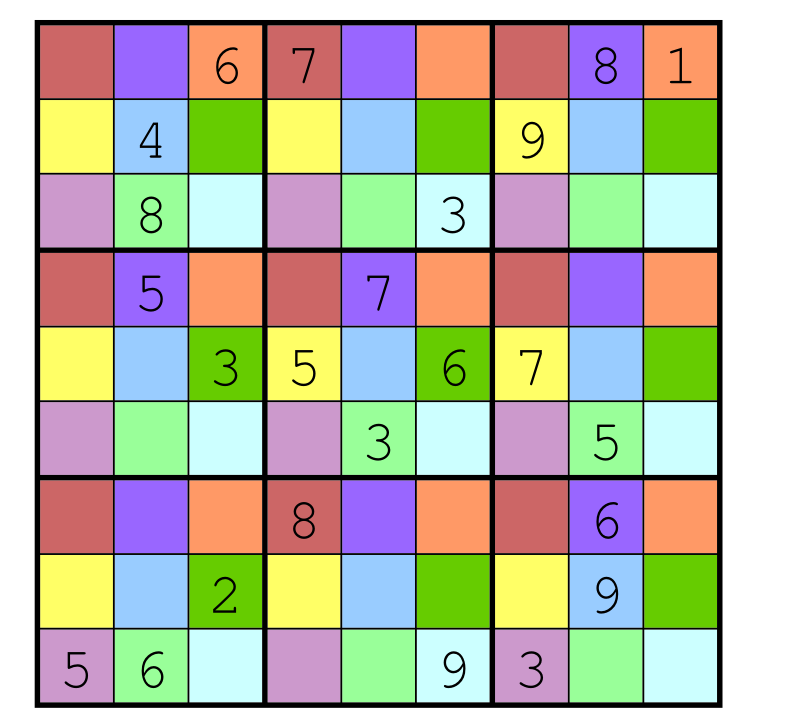
\includegraphics[scale=0.4]{Figures/positionSUDOKU.png}
	\caption{Παράδειγμα ενός Position SUDOKU παζλ. Κάθε κελί με το ίδιο χρώμα πρέπει να περιέχει όλους τους αριθμούς από το 1 εως και το 9 ακριβώς μία φορα τον καθέναν.}
\end{figure}

Η μαθηματική μοντελοποίηση θα περιλαμβάνει επιπλέον περιορισμούς, οι οποίοι δίνονται από τον πρακάτω τύπο: 

\begin{align*}
	\sum_{i=c}^{9}{\sum_{j=z}^{9} x_{ijk}} = 1 \quad c=1:(3):9 \quad j=1:(3):9 \quad \text{τα αθροίσματα προχωρούν με βήμα 3}
\end{align*}

Οπότε η τελική μορφή του προβλήματος βελτιστοποίησης είναι:

\begin{align*}
	\begin{aligned}
		\min &\quad 0^{T}x \\
		\textup{s.t.}\quad
		\sum_{i=1}^{9}x_{ijk} = 1 &\quad j=1:9, \quad k=1:9 \quad \text{μόνο ένα k σε κάθε στήλη του πίνακα} \\
		\sum_{j=1}^{9}x_{ijk} = 1 &\quad i=1:9, \quad k=1:9 \quad \text{μόνο ένα k σε κάθε γραμμή του πίνακα} \\
		\sum_{j=3q-3+1}^{3q} {\sum_{i=3p-3+1}^{3p}x_{ijk}} = 1 &\quad k=1:9, \quad p=1:3, \quad q=1:3 \quad \text{μόνο ένας ακέραιος k σε κάθε υποπίνακα} \\
		\sum_{k=1}^{9}x_{ijk} = 1 &\quad i=1:9, \quad j=1:9 \quad \text{όλα τα κελιά του πίνακα πρέπει να συμπληρωθούν} \\
		\sum_{i=c}^{9}{\sum_{j=z}^{9} x_{ijk}} = 1 &\quad c=1:(3):9 \quad j=1:(3):9 \quad k=1:9 \quad \text{κελιά με τις ίδιες συντεταγμένες σε όλους} \\ &\text{τους υποπίνακες έχουν μόνο ένα k} \\
		x_{ijk} = 1 \forall (i,j,k) \in G &\quad \text{τα κελιά του πίνακα που είναι συμπληρωμένα είναι "on"} \\
		x_{ijk} \in {0,1}&
	\end{aligned}
\end{align*}

\subsection{Three Magic SUDOKU}

Η παραλλαγή Three Magic SUDOKU υπάρχει ο επιπλέον κανόνας που ορίζει ότι στα σημειωμένα \(3 \times 3\) κουτιά (magic) οι 3 αριθμοί σε κάθε στήλη και οι 3 αριθμοί σε κάθε γραμμή αν αθροιστούν δίνουν το ίδιο αποτέλεσμα. Ένα παράδειγμα με 3 μαγικά κουτιά δίνεται στο Figure . Το πλήθος των μαγικών κουτιών μπορεί να ποικίλει. \par

\begin{mytheorem}{Three Magic SUDOKU}{}
	Οι κανόνες για το Three Magic SUDOKU σε έναν πίνακα μεγέθους \(9 \times 9\) με υποπίνακες μεγέθους \(3 \times 3\) είναι: \\
	\(\bullet\) Κάθε γραμμή του πίνακα μεγέθους 9 να περιέχει ακριβώς μια φορά κάθε ακέραιο αριθμό από το 1 ως το n. \\
	\(\bullet\) Κάθε στήλη του πίνακα μεγέθους 9 να περιέχει ακριβώς μια φορά κάθε ακέραιο αριθμό από το 1 ως το 9. \\
	\(\bullet\) Κάθε υποπίνακας μεγέθους \(3 \times 3\) να περιέχει ακριβώς μια φορά κάθε ακέραιο αριθμό από το 1 ως το 9. \\
	\(\bullet\) Σε κάθε μαγικό κουτί το άθροισμα των στηλών και των γραμμών πρέπει να είναι το ίδιο.
\end{mytheorem}

\begin{figure}[h]
	\centering	
	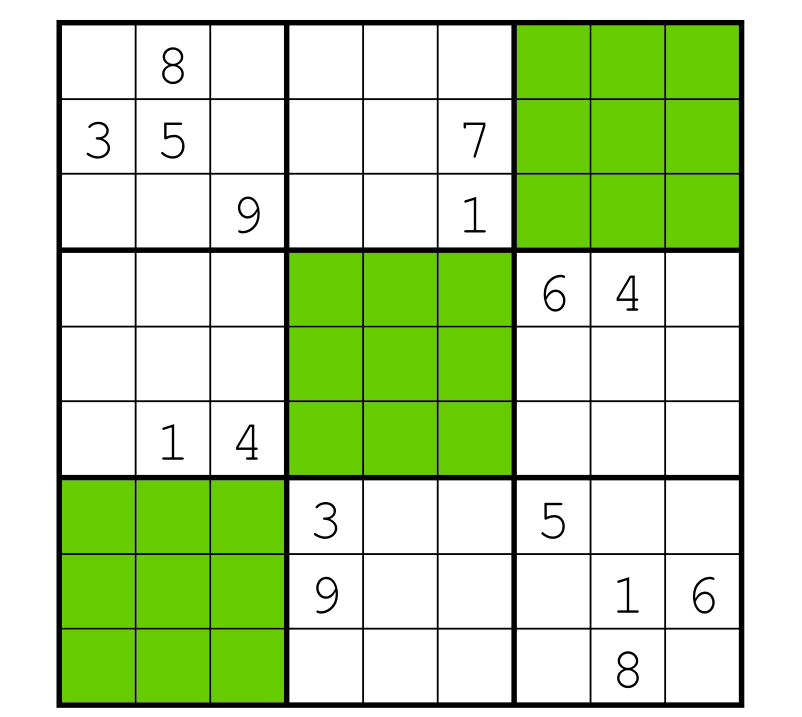
\includegraphics[scale=0.4]{Figures/threemagicSUDOKU.png}
	\caption{Παράδειγμα ενός Three Magic SUDOKU παζλ. Οι 3 αριθμοί σε κάθε στήλη και οι 3 αριθμοί σε κάθε γραμμή στα πράσινα \(3 \times 3\) κουτιά πρέπει αν προτεθούν να δίνουν τον ίδιο αριθμό.}
\end{figure}

Η μαθηματική μοντελοποίηση του Three Magic SUDOKU απαιτεί τον επιπλέον περιορισμό:

\begin{align*}
	...............
\end{align*}

Οπότε η τελική μορφή του προβλήματος βελτιστοποίησης είναι:

\begin{align*}
	\begin{aligned}
		\min &\quad 0^{T}x \\
		\textup{s.t.}\quad
		\sum_{i=1}^{9}x_{ijk} = 1 &\quad j=1:9, \quad k=1:9 \quad \text{μόνο ένα k σε κάθε στήλη του πίνακα} \\
		\sum_{j=1}^{9}x_{ijk} = 1 &\quad i=1:9, \quad k=1:9 \quad \text{μόνο ένα k σε κάθε γραμμή του πίνακα} \\
		\sum_{j=3q-3+1}^{3q} {\sum_{i=3p-3+1}^{3p}x_{ijk}} = 1 &\quad k=1:9, \quad p=1:3, \quad q=1:3 \quad \text{μόνο ένας ακέραιος k σε κάθε υποπίνακα} \\
		\sum_{k=1}^{9}x_{ijk} = 1 &\quad i=1:9, \quad j=1:9 \quad \text{όλα τα κελιά του πίνακα πρέπει να συμπληρωθούν} \\
		........ \\
		x_{ijk} = 1 \forall (i,j,k) \in G &\quad \text{τα κελιά του πίνακα που είναι συμπληρωμένα είναι "on"} \\
		x_{ijk} \in {0,1}&
	\end{aligned}
\end{align*}

\chapter{Δημιουργία SUDOKU παζλ}

Στο κεφάλαιο αυτό θα αναφερθούμε στους τρόπους με τους οποίους μπορούμε να δημιουργήσουμε SUDOKU παζλ.Αναφερόμαστε στα κριτήρια που οφείλει να ικανοποιεί ένας πίνακας SUDOKU, για να είναι επιλύσιμος, αλλά και για να προσελκύει τους λύτες. Αναφερόμαστε σε διάφορες τεχνικές για τη δημιουργία τέτοιων παζλ, που έχουν κατά καιρούς ακολουθηθεί από δημιουργούς SUDOKU, αλλά και ερευνητές, που έχουν καταπιαστεί με το ζήτημα. Αναλύουμε την απλή bruteforce μέθοδο κι έπειτα συζητάμε τη δημιουργία παζλ από προγενέστερα παζλ. Δίνουμε μία βασική μαθηματική προσέγγιση στο ζήτημα, για να ισχυροποιήσουμε την ορθότητα των τεχνικών. \par

\section{Κριτήρια SUDOKU παζλ}

Ένα καλό παζλ SUDOKU οφείλει να πληρεί ορισμένες βασικές προϋποθέσεις, για να έχει λύση, αλλά και για να επιθυμεί κάποιος πιθανός λύτης να ενασχοληθεί με αυτό. Τα κριτήρια αυτά, όπως παραθέτονται στο \cite{9} είναι: \\
\(\bullet\) Το SUDOKU παζλ πρέπει να έχει μοναδική λύση. \\
\(\bullet\) Να μην απαιτεί από τον λύτη να μπαίνει σε διαδικασία να μαντέψει αν η λύση είναι σωστή ή όχι μία δεδομένη στιγμή. Στην πραγματικότητα, αυτό που θέλει ο άνθρωπος όταν λύνει ένα SUDOKU είναι να έχει στη διάθεση του μεθόδους που να δηλώνουν με σιγουριά αν η τοποθέτηση (ή αντίστοιχα η απόρριψη) του αριθμού  που πραγματοποιούν σε μία δεδομένη στιγμή του παιχνιδιού είναι ορθή. Φυσικά, κανείς ακόμη δεν έχει φτάσει σε επίπεδο τα SUDOKU παζλ που δημιουργεί να μην απαιτούν ποτέ την επίκληση της τύχης για την επιλογή αριθμού που θα γεμίσει κάποιο κελί. Ωστόσο, αυτό είναι κάτι που καλό είναι να αποφεύγουμε όταν γινόμαστε δημιουργοί SUDOKU. \\ 
\(\bullet\) Το SUDOKU παζλ πρέπει να κατατάσσεται ορθά σε επίπεδα δυσκολίας και αυτό είναι ίσως ένα από τα πίο δύσκολα εγχειρήματα στη φάση δημιουργιας τέτοιων παζλ. Είναι συχνό φαινόμενο κάποιος να αξιολογεί το ίδιο παζλ ως προς το επίπεδο δυσκολίας με πολύ διαφορετικό τρόπο από κάποιον άλλον. Έχουμε αναφερθεί πιο αναλυτικά στην αξιολόγηση των SUDOKU παζλ στο αντίστοιχο κεφάλαιο. \\
\(\bullet\) Ένα SUDOKU παζλ πρέπει να έχει το ίδιο διαβαθμιση δυσκολίας κατά τη διαδικασία επίλυσής του. Πιο συγκεκριμένα, ακόμα και στα παζλ δύσκολου επιπέδου, ο μέσος λύτης πρέπει να μπορεί να συμπληρώνει τα πρωτα ~10 κελιά του πίνακα σχετικά εύκολα. Αντίστοιχα, η συμπλήρωση των ~10-15 τελευταίων κελιών πρέπει να είναι η πιο απαιτητική συμπλήρωση μέχρι εκείνη τη στιγμή της έκβασης της διαδικασίας επίλυσης. \\
\(\bullet\) Το SUDOKU παζλ πρέπει να έχει απλή μορφή. Καλό είναι να περιέχει όσο λιγότερα δεδομένα ψηφία γίνεται. Έχει αποδειχθεί μαθηματικά πως το μέγιστο πλήθος αριθμών που απαιτείται για την εύρεση της επίλυσης ενός παζλ SUDOKU είναι 39 και το ελάχιστο είναι 17. \\
\(\bullet\) Το τελευταίο κριτήριο, δεν είναι τόσο σημαντικό, καθώς δε σχετίζεται με την ουσία του παζλ. Είναι καλό να προσέχουμε το SUDOKU να είναι συμμετρικό, καθώς αυτό το κάνει πιο ελκυστικό στο ανθρώπινο μάτι. \par


\section{Δημιουργία SUDOKU παζλ με bruteforce}

Μία πρώτη προσέγγιση για τη δημιοργία ενός παζλ SUDOKU είναι το bruteforce. Σε έναν πίνακα μεγέθους \(n \times n\) τοποθετούμε τυχαία αριθμούς από το 1 ως το n στα κελιά του και στη συνέχεια ελέγχουμε αν ο τελικός πίνακας που προκύπτει συμμορφώνεται με τους κανόνες που αναφέρονται στον Ορισμό 5.3.1. \par

Η τεχνική αυτή δημιουργεί περίπου \(n^{n^2}\) διαφορετικούς πίνακες. Αν αναφερόμαστε σε πίνακα μεγέθους \(9 \times 9\), τότε ο αριθμός αυτός προσεγγίζει τους \(1.97\times10^{77}\) διαφορετικούς πίνακες. \par 

Το ερώτημα είναι πόσοι από αυτούς τους πίνακες συμμορφώνονται με τους κανόνες του Ορισμού 5.3.1. \par

Από το \cite{6} γνωρίζουμε ότι τα \(9 \times 9\) Latin squares είναι \(5.525\times10^{27}\) το πλήθος και αφού τα κλασσικά SUDOKU είναι ειδικές περιπτώσεις των Latin squares, ο αριθμός τους θα είναι μικρότερος από \(5.525\times10^{27}\). Τελικά, ο αριθμός των κλασσικών παζλ υπολογίστηκε στο \cite{7} το 2005 να είναι περίπου \(6.67\times10^{21}\). Αν ληφθούν υπόψη και οι συμμετριές, τότε ο αριθμός μειώνεται αισθητά \cite{8}.

Αν υποθέσουμε ότι ξεπερνάμε τους μεγάλους αριθμούς διαφορετικών πινάκων και σταματάμε την αναζήτηση valid πίνακα με το που βρούμε τον πρώτο. Είναι σημαντικό να γνωρίζουμε ποιος είναι ο ελάχιστος αριθμός δεδομένων κελιών (τα κελιά που περιέχουν αριθμούς στη αρχή), ώστε να καταφέρει ο παίκτης με βάση αυτά να φτάσει στη μοναδική λύση. Σε γενικές γραμμές δεν υπάρχει θεωρητική προσέγγιση που να απαντά σε αυτό το ερώτημα πλήρως, παρά μόνο πειραματικές προσεγγίζεις. Σίγουρα, οι πειραματικές προσεγγσεις υποδεικνύουν ότι χρειάζονται τουλάχιστον 17 κελιά συμπληρωμένα. Φυσικά, όσα περισσότερα δεδομένα κελιά δίνονται, τόσο πιο εύκολο γίνεται το παζλ. Η δυσκολία επίλυσης ενός παζλ καθορίζεται και από τη θέση των δεδομένων κελιών, αλλά και των τιμών που παίρνουν τα δεδομένα κελιά.

\section{Δημιουργία SUDOKU παζλ από προγενέστερα παζλ}

Στην παρούσα υποενότητα θα αναφερθούμε στον τρόπο με τον οποίο μπορούμε να δημιουργήσουμε νέα παζλ βασισμένοι σε κάποιο άλλο SUDOKU παζλ. Για να το επιτύχουμε αυτό πρέπει να διατυπώσουμε μερικούς μαθηματικούς ορισμούς και θεωρήματα. \par

Τα καινούρια SUDOKU που επιθυμούμε να δημιουργήσουμε από κάποιο προγενέστερο SUDOKU πρέπει να πληρούν ορισμένες προϋποθέσεις, για να είναι έγκυρα. Οι προϋποθέσεις αυτές σχετίζονται με το μέγεθος του παζλ και τους βασικούς κανόνες που αναφέρονται σε ένα κλασσικό παιχνίδι SUDOKU. Συνοψίζουμε τις πρϋποθέσεις για έναν πίνακα SUDOKU στον παρακάτω ορισμό. \par

\begin{mytheorem}{SUDOKU πίνακας}{}
	Ένας τετραγωνικός πίνακας \(S\) είναι SUDOKU πίνακας αν ισχύουν τα παρακάτω: \\
	\(\bullet\) Αν το μέγεθος του πίνακα είναι \(n\), τότε θα πρέπει να ισχύει ότι \(n = m^{2}\) , όπου το \(m\) μπορεί να είναι οποιοσδήποτε θετικός ακέραιος αριθμός. \\
	\(\bullet\) Κάθε γραμμή του πίνακα μεγέθους \(n\) να περιέχει ακριβώς μια φορά κάθε ακέραιο αριθμό από το 1 ως το n. \\
	\(\bullet\) Κάθε στήλη του πίνακα μεγέθους \(n\) να περιέχει ακριβώς μια φορά κάθε ακέραιο αριθμό από το 1 ως το 9. \\
	\(\bullet\) Κάθε υποπίνακας μεγέθους \(m \times m\) να περιέχει ακριβώς μια φορά κάθε ακέραιο αριθμό από το 1 ως το n. \\
\end{mytheorem}

Σκοπός μας είναι να καταφέρουμε από ένα SUDOKU παζλ, έστω το \(S\) να κατασκευάσουμε όσα περισσότερα νέα παζλ που να προέρχονται από το \(S\), αλλά ταυτόχρονα να διαφέρουν από αυτό. Άρα, αν \(S\) είναι το αρχικό παζλ, από το οποίο θα προκύψουν τα καινούρια παζλ και \(\overline{S}\) τα νέα παζλ, τότε πρέπει να ισχύει ότι: 

\begin{align}
	\overline{S} \neq S \Leftrightarrow 
	\overline{S} - S \neq 0
\end{align}

Μία πολύ απλή προσέγγιση, που από ενα παζλ \(S\) θα καταλήξουμε σε ένα νέο παζλ \(\overline{S}\) είναι να αντιστρέψουμε τον πίνακα \(S\), οπότε για τον νέο πίνακα που θα προκύψει, θα ισχύει η σχέση (6.1). Διατυπώνουμε τη σκέψη αυτή ως θεώρημα. \par

\begin{theorem}{}{}
	Αν ο \(S\) είναι ένας πίνακα SUDOKU, τότε και ο \(S^{T}\) είναι πίνακας SUDOKU.
\end{theorem}

Απόδειξη: \\
Για να αποδείξουμε το θεώρημα πρέπει να δείξουμε ότι για τον \(S^{T}\) ισχύουν οι προϋποθέσεις του ορισμού 6.0.1. \\ \\

Έστω ότι ο πίνακας \(S\) είναι μεγέθους \(n \times n\) τέτοιο ώστε \(n = m^2\). Αν τον αντιστρεψουμε, τότε και ο \(S^{T}\) θα είναι μεγέθους \(n \times n\). Συνεπώς το πρώτο κριτήριο του Ορισμού 6.0.1 ισχύει. \\ \\

Κατά την αντιστροφή οι γραμμές του \(S\) γίνονται στήλες στον \(S^{T}\) και οι στήλες γραμμές. Έτσι, 

\begin{align*}
	S^{T}_{ij} = S_{ji}
\end{align*}

Στον \(S\) ισχύει ότι "Κάθε γραμμή του πίνακα περιέχει ακριβώς μια φορά κάθε ακέραιο αριθμό από το 1 ως το n", άρα στον \(S^{T}\) αυτό σημαίνει ότι "Κάθε στήλη του πίνακα περιέχει ακριβώς μια φορά κάθε ακέραιο αριθμό από το 1 ως το n". Αντίστοιχα, στον \(S\) ισχύει ότι "Κάθε στήλη του πίνακα περιέχει ακριβώς μια φορά κάθε ακέραιο αριθμό από το 1 ως το n", άρα στον \(S^{T}\) θα ισχύει ότι "Κάθε στήλη του πίνακα περιέχει ακριβώς μια φορά κάθε ακέραιο αριθμό από το 1 ως το n". Άρα, το δέυτερο και το τρίτο κριτήριο που θέσαμε στον Ορισμό 6.0.1 ικανοποιούνται και για τον \(S^{T}\). \\ \\ 

Για το τελευταίο κριτήριο, θα υποθέσουμε χωρίς βλάβη της γενικότητας ότι αναφερόμαστε σε έναν πίνακα SUDOKU μεγέθους \(4 \times 4\), άρα \(m = 2\). Αν για τον πίνακα \(S\) ισχύει ότι: 

\begin{align*}
	S = \begin{pmatrix}
		S_{11} & S_{12} \\
		S_{21} & S_{22}
	\end{pmatrix}
\end{align*}

όπου ως \(S_{ij}\) συμβολίζονται οι υποπίνακες του \(S\), τότε για τον \(S^{T}\) θα ισχύει ότι: 

\begin{align*}
	S = \begin{pmatrix}
		S_{11}^{T} & S_{21}^{T} \\
		S_{12}^{T} & S_{22}^{T}
	\end{pmatrix}
\end{align*}

Όλοι οι υποπίνακες του \(S^{T}\) κατασκεαύστηκαν από τους υποπίνακες του \(S\) και συνεπώς ικανοποιείται και η τελευταία προϋπόθεση του Ορισμού 6.0.1. \(\square\)

Ωστόσο, με το Θεώρημα 6.0.1 μπορούμε να κατασκεύασουμε μόνο έναν πίνακα από έναν άλλον. Σκοπός μας είναι να επιτύχουμε πολλά περισσότερα από αυτό. Σκοπός μας είναι να καταφέρουμε να κατασκευάζουμε πολλά νέα παζλ από ένα προγενέστερο παζλ. 

\begin{theorem}{}{}
	Αν \(S\) είναι ένας πίνακας SUDOKU, τότε ένας νεός πίνακα SUDOKU \(\overline{S}\) μπορεί να δημιουργηθεί αλλάζοντας τη θέση σε γραμμές και στήλες σε επίπεδο υποπίνακα.
\end{theorem}

Απόδειξη: \\
Χωρίς βλάβη της γενικότητας υποθέτουμε ότι αναφερόμαστε σε πίνακες SUDOKU μεγέθους \(4 \times 4\), άρα \(n = 4\) και \(m = 2\). Η αλλαγή θέσης σε γραμμές και στήλες σε επίπεδο υποπίνακα μπορεί να περιγραφεί από την παρακατω σχέση, με τα \(E_{i}\) και τα \(F_{i}\) να είναι μεταθετικοί πίνακες, δηλαδή πίνακε ςπου αλλάζουν τη σειρά των γραμμών (ή των στηλών): 

\begin{align*}
	\overline{S} &= \begin{pmatrix}
						E_{1} &  \\
							  & E_{2}
	\end{pmatrix}
	\begin{pmatrix}
		S_{11} & S_{12} \\
		S_{21} & S_{22}
	\end{pmatrix}
	\begin{pmatrix}
		F_{1} &  \\
		& F_{2}
	\end{pmatrix} \Leftrightarrow \\
	\overline{S} &= \begin{pmatrix}
						E_{1}S_{11}F_{1} & E_{1}S_{12}F_{2} \\
						E_{2}S_{21}F_{1} & E_{2}S_{22}F_{2}
					\end{pmatrix}
\end{align*}

Και σε αυτήν την απόδειξη, πρέπει να ελέγξουμε αν ισχύουν και οι τέσσερις προϋποθέσεις που αναφέραμε στον Ορισμό 6.0.1, ώστε το Θεώρημα να ισχύει. \\ \\ 

Προφανώς, η παραπάνω αλλαγή δεν επεμβαίνει στο μέγεθος του καινούριο πίνακα, συνεπώς η πρώτη προϋπόθεση του ορισμού 6.0.1 ισχύει. \\ \\ (................)

\(\square\)

Ένας ακόμη τρόπος για να δημιουργησουμε νέα παζλ SUDOKU είναι να αλλάξουμε, με συγκεκριμένη τεχνική, τους ακεραίους του SUDOKU που ήδη διαθέτουμε. \par 

\begin{theorem}{}{}
	Αν \(S\) είναι ένας πίνακας SUDOKU, τότε ένας νεός πίνακα SUDOKU \(\overline{S}\) μπορεί να δημιουργηθεί αλλάζοντας τους ακέραιους αριθμούς του \(S\), με ένα προς ένα αντιστοίχιση ανάμεσα στο σύνολο α = \(\left( 1,2,\dots,n\right)\) που κατασκευάζει το \(S\) και στο σύνολο β, που είναι υπεύθυνο για την κατασκευή του \(\overline{S}\) και είναι μία μετάθεση του συνόλου α.
\end{theorem}

Απόδειξη: \\
Υποθέτουμε ότι \(α \neq β\) και ότι ο \(\overline{S}\) δεν είναι ένας νέος πίνακας SUDOKU. \\

Χωρίς βλάβη της γενικότητας υποθέτουμε ότι ο \(\overline{S}\) δεν ικανοποιεί το δεύτερο κριτήριο του Ορισμού 6.0.1, άρα υπάρχει γραμμή που περιλαμβάνει δύο ή περισσότερες φορές έναν ακέραιο και παραλείπει κάποιον/-ους άλλον/-ους. Αυτό, προφανώς σημαίνει ότι η αντιστόιχιση από το α στο β δεν είναι ένα προς ένα. Συνεπώς, το \(\overline{S}\) είναι ένας νέος πίνακας SUDOKU. \(\square\)

\section{Δημουργία SUDOKU παζλ βάση λογικών στρατηγικών}

Μία εντολώς διαφορετική προσέγγιση για τη δημιουργία SUDOKU παζλ, που είναι πιο αφηρημένη και όχι τόσο μαθηματική γίνεται με τη χρήση λογικών στρατηγικών. Ο Andrew C. Stuart στο \cite{9} ακολούθησε μία τέτοια προγέγγιση. \par

Για τη δημιουργία ενός νέου παζλ πρέπει πρώτα γνωρίζουμε τη λύση του, συνεπώς πρέπει να κατασκευάσουμε τον πίνακα και να τον συμπληρώσουμε με όλους τους αριθμούς από το 1 ως το n, με τέτοιον τρόπο ώστε να ικανοποιούνται οι προϋποθέσεις του Ορισμού 3.0.1. Για τη συμπλήρωση του πίνακα χρησιμοποιήθηκαν στρατηγικές βασισμένες στη λογική. \par

Πρώτο βήμα της διαδικασίας είναι η συμπλήρωση, με τυχαίο τρόπο, n κελιών του πίνακα με αριθμούς από το 1 ως το n, κάνοντας χρήση του κάθε αριθμού ακριβώς μία φορά. Έπειτα, αποφασίζεται για κάθε κελί ποιο είναι το κατάλληλο ψηφίο που πρέπει να είναι εκεί τοποθετημένο εκεί. Αυτό ενέχει στοιχεία τύχης και για αυτόν το λόγο αν καταλήξουμε σε αδιέξοδο πρέπει να υπάρχει τρόπος να ανακαλέσουμε αυτήν την επιλογή που προκάλεσε προβληματική συμπεριφορά και να συνεχίσουμε εκ νέου τη διαδικασία. \par

Έχοντας πλέον έναν πλήρως συμπληρωμένο πίνακα, ξεκινά η διαδικασία αφαίρεσης ψηφίων από τον πίνακα, για να οδηγηθούμε στη τελική μορφή του παζλ. Αφαιρούνται δύο ή τέσσερις αριθμοί κάθε φορά, που είναι διαγωνίως αντίθετοι. Στις πρώτες είκοσι αφαιρέσεις μπορούμε να αφαιρούμε τετράδες αριθμών, ενώ στη συνέχεια τα πράγματα γίνονται πιο αυστηρά και καταφεύγουμε στα ζευγάρια αριθμών. Φυσικά, έπειτα από κάθε αφαίρεση τετράδας ή ζευγαριού ελέγχεται αν το προκύπτον παζλ είναι επιλύσιμο, αλλιώς επανατοποθετούμε την τετράδα ή το ζεύγος αντίστοιχα και συνεχίζουμε τη διαδικασία. Όπως έχουμε προαναφέρει, δε μπορούμε να καταλήξουμε σε πίνακα με λιγότερα από 17 συμπληρωμένα κελιά και αν προκύψει πίνακας με περισσότερα από 39 συμπληρωμένα κελιά, τότε οφείλουμε να συνεχίσουμε τη διαδικασία αφαίρεσης ψηφίων από το παζλ, καθώς το προκύπτον παζλ θα είναι εξαιρετικά εύκολο. \par

\chapter{Επίπεδα δυσκολίας SUDOKU παζλ}

Στο παρόν κεφάλαιο θα μελετήσουμε τις τεχνικές που χρησιμοποιούνται από τον άνθρωπο για την επίλυση ενός SUDOKU παζλ και θα επιχειρήσουμε να μετρήσουμε τα επίπεδα δυσκολίας ενός τέτοιου παζλ. Δεν έχουν αναπτυχθεί ακόμη εφαρμόσιμες θεωρίες, που μπορούν να βοηθήσουν προς αυτήν την κατεύθυνση. Χωρίς βλάβη της γενικότητας στο κεφάλαιο αυτό όποτε αναφερόμαστε σε παζλ SUDOKU θα εννοούμε μεγέθους \(4 \times 4\), γιατί διευκολύνει τη μελέτη μας, εκτός αν αναφέρεται ρητά κατί διαφορετικό. \par

\section{Μελέτη των επιπέδων δυσκολίας στην επίλυση SUDOKU παζλ από τον άνθρωπο}

Το ζήτημα του προσδιορισμού των επιπέδων δυσκολίας για παζλ SUDOKU απασχολεί όχι μόνο τους δημιουργούς αυτών των παζλ, αλλά και τους ίδιους του παίκτες. Πώς ακριβώς προσδιορίζεται το επίπεδο δυσκολίας ενός παζλ; Μέχρι και σήμερα δεν υπάρχουν θεωρητικές προσεγγίσεις στις οποίες μπορούμε να βασιστούμε με σιγουριά για να απαντήσουμε το συγκεκριμένο ερώτημα. \par 

Σύμφωνα με τη μελέτη \cite{5} υπάρχουν δύο προσεγγίσεις του προβλήματος. Η πρώτη έχει να κάνει με την πολυπλοκότητα των ανεξάρτητων βημάτων που οδηγούν στη λύση του παζλ. Αυτή είναι η πιο συνηθισμένη προσέγγιση που χρησιμοποιείται για την εκτίμηση του επιπέδου δυσκολίας των παζλ. Η δεύτερη σχετίζεται με το αν τα βήματα που οδηγούν στη λύση είναι ανεξάρτητα ή οχι. \par

Ορίζουμε το πρόβλημα επίλυσης SUDOKU παζλ ως πρόβλημα ικανοποίησης περιορισμών, απόφαση που έχει ερμηνευτεί λεπτομερέστερα σε προηγούμενο κεφάλαιο. Υπάρχουν δύο προσεγγίζεις για την επίλυση ενός προβλήματος απόφασης για SUDOKU παζλ, η backtracking και η constraint propagation. \par

Το backtracking είναι ουσιαστικά ένας bruteforce τρόπος επίλυσης προβλημάτων περιορισμών. Ξεκινά με μία κενή ανάθεση τιμών στις μεταβλητές τους προβλήματος και αναθέτοντας τιμές τη μία μετά την άλλη επιχειρεί να καταλήξει σε λύση. Η τεχνική αυτή είναι σίγουρο πως θα καταλήξει σε λύση, αφού ουσιαστικά ελέγχει όλους τους πιθανούς τρόπους με τους οποίους μπορεί να συμπληρωθεί ένα παζλ. \par

Παζλ μεγέθους \(9 \times 9\) ο υπολογιστής είναι σε θέση να τα επιλύει με αυτήν την τεχνική σχετικά εύκολα. Ωστόσο, για τον άνθρωπο αυτή η προσέγγιση είναι ιδιαίτερα κουραστική και σίγουρα καθόλου διασκεδαστική, γι'αυτο και δεν προτιμάται σε καμμία περίπτωση. \par

\begin{figure}[h]
	\centering	
	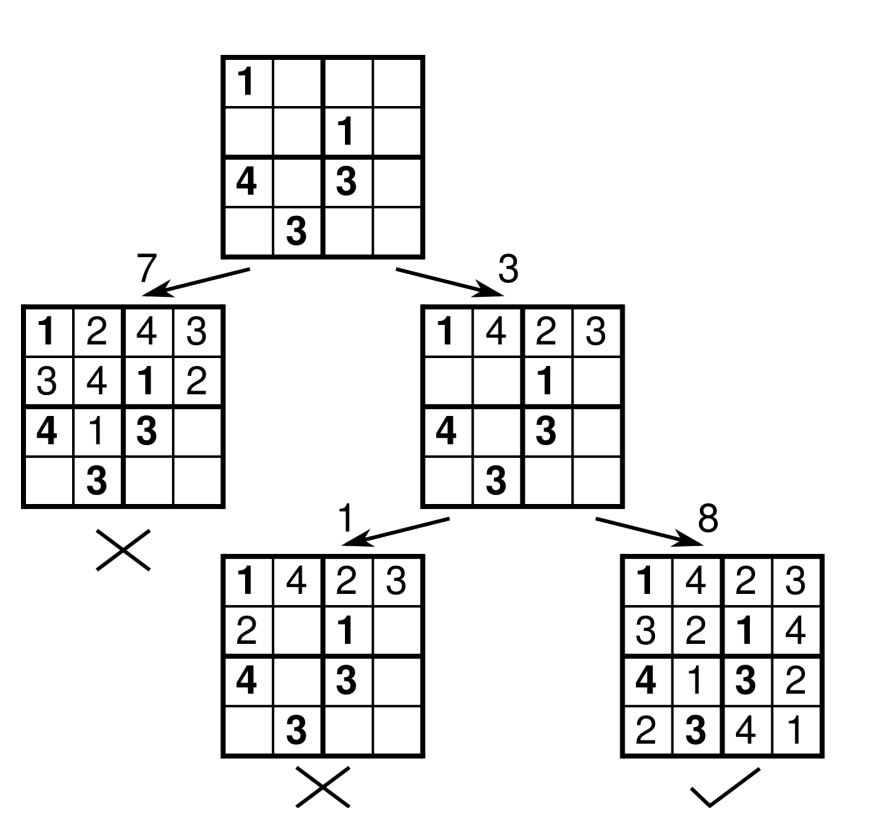
\includegraphics[scale=0.45]{Figures/backtracking.png}
	\caption{Μέρος της διαδικασίας επίλυσης ενός \(4 \times 4\) SUDOKU με την τεχνική backtracking}
\end{figure}

Με την constraint propagation τεχνική χρησιμοποιούμε τη λογική για να για να βρούμε την τιμή κάποιων μεταβλητών, εξετάζοντας τους περιορισμούς. Για κάθε μεταβλητή ορίζουμε ένα σύνολο τιμών που μπορεί να λάβει χωρίς να προκαλέσει την παραβίαση κανενός περιορισμού. \par

Η τεχική αυτή δεν είναι βέβαιο πως θα οδηγήσει σε λύση, αλλά σίγουρα είναι πιο αποδοτική. Μπορεί να συνδυαστεί με backtracking για καλύτερα αποτελέσματα. Το constraint propagation είναι η τεχνική που χρησιμοποιεί ο ανθρώπινος εγκέφαλος για να επιλύσει ένα SUDOKU παζλ. \par

\begin{figure}[h]
	\centering	
	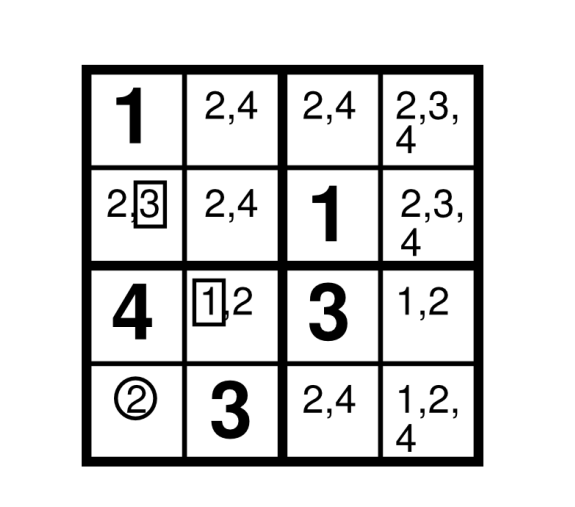
\includegraphics[scale=0.45]{Figures/propagation.png}
	\caption{Μέρος της διαδικασίας επίλυσης ενός \(4 \times 4\) SUDOKU με την τεχνική constraint propagation}
\end{figure}

Συγκεκριμένα ο άνθρωπος χρησιμοποιεί δύο είδη τεχνικών για να επιλύσει το παζλ: η Naked single technique (ή αλλιώς singleton, single value, forced value, exclusion
principle), όπου για ένα δεδομένο κελί του πίνακα υπάρχει μόνο μία τιμή που μπορεί να ανατεθεί, καθώς όλες οι υπόλοιπες τιμές πλήττουν κάποιον περιορισμο και η Hidden single technique (ή αλλιώς naked value, inclusion principle), όπου για μία συγκεκριμένη γραμμή ή στήλη ή για έναν συγκεκριμένο υποπίνακα του παζλ υπάρχει μόνο ένα κελί που μπορεί να φιλοξενήσει μία συγκεκριμένη τιμή. \par

Το πείραμα που πραγματοποιήθηκε για να συσχετίσει τη συμπεριφορά των ανθρώπων απέναντι σε παζλ, ώστε να προκύψουν συμπεράσματα για τα επίπεδα δυσκολίας τους στο \cite{5} αντλεί δεδομένα από τον παγκόσμιο ιστό. Καθώς το SUDOKU είναι ένα ευρέως διαδεδομένο παιχνίδι, υπάρχει πληθώρα δεδομένων στον παγκόσμιο ιστό που με κατάλληλη επεξερασία φάνηκαν χρήσιμα στην έρευνα. Φυσικά, τέτοια δεδομένα δεν είναι τα πλέον κατάλληλα, καθώς δεν υπόκεινται σε εργαστηριακόυς κανόνες, ωστόσο η πληθώρα τους τα κάνει εξίσου σημαντικά. \par

Ως μέτρο για την εκτίμηση την δυσκολίας των ανθρώπων να λύσουν ένα παζλ SUDOKU χρησιμοποιήθηκε ο μέσος χρόνος επίλυσης.

Αν πρέπει να ορίσουμε λίγο πιο αυστηρά το μοντέλο που χρησιμοποιεί ο άνθρωπος για την επίλυση SUDOKU, πρέπει να γίνουν ορισμένες παραδοχές. Ο άνθρωπος δεν είναι καλός στη συστηματική αναζήτηση, γι'αυτό και τεχνικές όπως το backtracking δεν τις προτιμα, όπως αναφέραμε προηγουμένως. Προτιμά να λύνει τέτοιου είδους προβλήματα με όσο το δυνατό πιο απλές λογικές τεχνικές όπως το constrait propagation. Επίσης, πρέπει να υποθέσουμε ότι κατά τη διαδικασία την επίλυσης του παζλ δε συμβαίνουν λάθη και ότι πάντα μπορεί να υπάρξει και επόμενο βήμα, μέχρι να φτάσουμε στη λύση. \par 

Το ανθρώπινο μοντέλο επίλυσης SUDOKU δίνεται παρακάτω: 

\begin{mytheorem}{Επίλυση SUDOKU από τον άνθρωπο}{}
	\(\bullet\) L είναι η πιο απλή τεχνική που μπορεί να προκαλέσει θετική έκβαση στην επίλυση του παζλ. \\
	\(\bullet\) Επιλογή του τρόπου (αν υπάρχουν πολλοί) που θα εφαρμοστεί το L στην τρέχουσα κατάσταση. \\
	\(\bullet\) Εφαρμογή. \\
\end{mytheorem}

Η αξιολόγηση του μοντέλου έγινε συγκρίνοντας τα δεδομένα των ανθρώπων που προέρχονταο από τον παγκόσμιο ιστό και τα δεδομένα από το μοντέλο. Χρησιμοποιήθηκαν 15 διαφορετικής δυσκολίας παζλ και κάθε παζλ επιλύθηκε από 10 εως και 60 άτομα. Τα αποτελέσματα αυτή της συσχέτισης φαίνονται στο Figure . \par

\begin{figure}[h]
	\centering	
	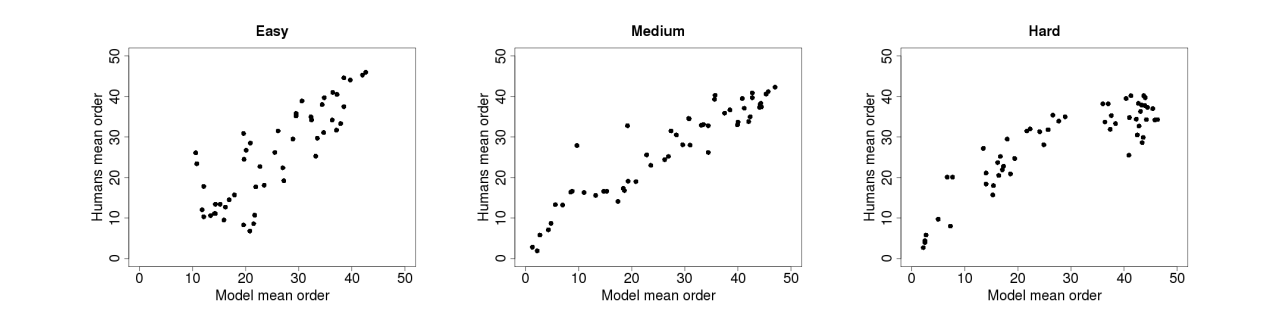
\includegraphics[scale=0.4]{Figures/results.png}
	\caption{Αποτελέσματα του πειράματος \cite{5}}
\end{figure}

Τελικά, η έρευνα \cite{5} καταλήγει στο συμπέρασμα ότι μπορούμε να βρούμε αρκετά καλές μετρικές για τα επίπεδα δυσκολίας ενός SUDOKU, ειδικά αν στη μοντελοποίηση λάβουμε υπόψη και ειδικά θέματα που σχετίζονται αποκλειστικά και μόνο με το SUDOKU ως παιχνίδι. 

\section{Στατιστική προσέγγιση}

Στο \cite{9} πραγματοποιήθηκε μελέτη του ζητήματος της ταξινόμησης των SUDOKU παζλ ανάλογα με το επίπεδο δυσκολίας τους, με πραγματικά δεδομένα. Τα εν λόγω δεδομένα ήταν ορθές καταχωρήσεις λυμένων παζλ από χρήστες του Διαδικτύου σε ένα καθημερινό διαγωνισμό για SUDOKU. Έτσι, καθημερινά συγκεντρώνονταν 2000 με 3000 καταχωρήσεις σωστά λυμένων παζλ. Τα επίπεδα δυσκολίας ήταν από πριν καθορισμένα και η μελέτη αυτή ήρθε να επιβεβαιώση την κατηγοριοποίηση τους σε "Gentle", "Moderate", "Tough" και "Diabolical" \par

Αφού οι άνθρωποι έλυναν κάποιο/-α παζλ έπειτα έπρεπε να δηλώσουν τον χρόνο που χρειάστηκαν, για να καταφέρουν να φτάσουν στη λύση. Η επιλογή έγινε από συγκεκριμένα χρονικά διαστήματα: \\
\(\bullet\) λιγότερα από 5 λεπτά, \\
\(\bullet\) περισσότερο από 5 λεπτά και λιγότερα από 10 λεπτά, \\
\(\bullet\) περισσότερο από 10 λεπτά και λιγότερα από 15 λεπτά, \\
\(\bullet\) περισσότερο από 15 λεπτά και λιγότερα από 20 λεπτά, \\
\(\bullet\) περισσότερο από 20 λεπτά και λιγότερα από 30 λεπτά, \\
\(\bullet\) περισσότερο από 30 λεπτά και λιγότερα από 40 λεπτά, \\
\(\bullet\) περισσότερο από 40 λεπτά και λιγότερα από 50 λεπτά, \\
\(\bullet\) περισσότερο από 50 λεπτά και λιγότερα από 60 λεπτά, \\
\(\bullet\) περισσότερο από 60 λεπτά και λιγότερα από 120 λεπτά, \\
\(\bullet\) περισσότερο από 120 λεπτά \\
\(\bullet\) δεν επιθυμώ να απαντήσω \ δε γνωρίζω \\

Οι απαντήσεις με την τελευταία επιλογή απορρίπτονταν.  /par

Στο Figure παρατίθενται το πλήθος των λύσεων για 330 παζλ, για κάθε χρονικό διάστημα επίλυσης και κάθε βαθμό.

\begin{figure}[h]
	\centering	
	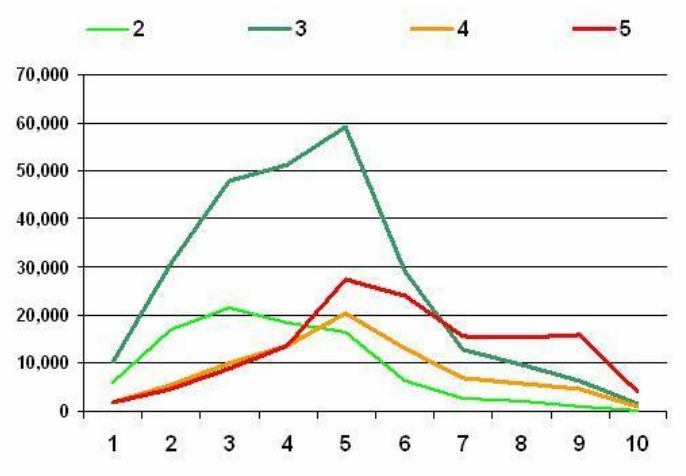
\includegraphics[scale=0.45]{Figures/stat1.png}
	\caption{Γράφημα της στατιστικής μελέτης για την ταξινόμηση των SUDOKU ανάλογα με το επίπεδο δυσκολίας τους. Gentle = ανοιχτό πράσινο, Moderate = σκούρο πράσινο, Tough = κίτρινο, Diabolical = κόκκινο}
\end{figure} 

Στο επόμενο Figure καταγράφονται οι μέσοι χρόνοι επίλυσης σε λεπτά για κάθε επίπεδο δυσκολίας. Το παράθυρο του χρόνου εδώ είναι από 16 λεπτά μέχρι και λίγο περισσότερα από μία ώρα. Είναι φανερό πως τα "Gentles" λύθηκαν σε λιγότερο χρόνο, ενώ τα "Diabolicals" το αντίθετο. Όσο για τα "Tough's" φαίνεται πως διχάζουν το κοινό ως προς τη δυσκολία τους.

\begin{figure}[h]
	\centering	
	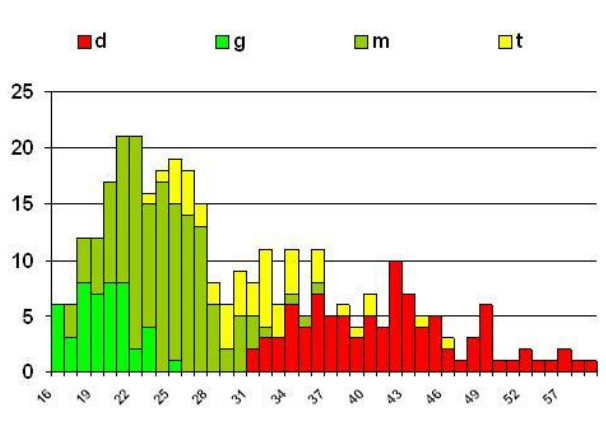
\includegraphics[scale=0.55]{Figures/stat2.png}
	\caption{Γράφημα της στατιστικής μελέτης για την ταξινόμηση των SUDOKU ανάλογα με το επίπεδο δυσκολίας τους . Gentle = ανοιχτό πράσινο, Moderate = σκούρο πράσινο, Tough = κίτρινο, Diabolical = κόκκινο}
\end{figure} 

\begin{figure}[h]
	\centering	
	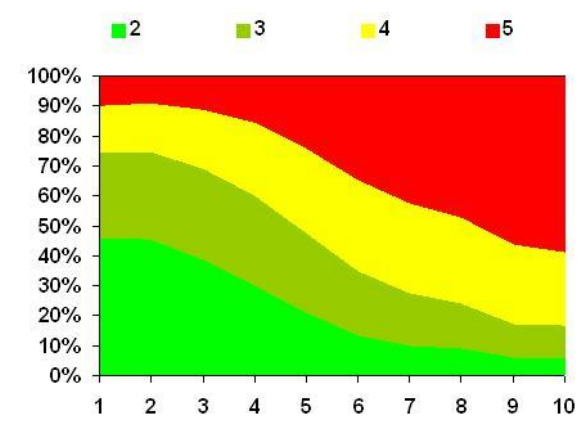
\includegraphics[scale=0.55]{Figures/stat3.png}
	\caption{Γράφημα της στατιστικής μελέτης για την ταξινόμηση των SUDOKU ανάλογα με το επίπεδο δυσκολίας τους . Gentle = ανοιχτό πράσινο, Moderate = σκούρο πράσινο, Tough = κίτρινο, Diabolical = κόκκινο}
\end{figure} 

Το διάγραμμα στο Figure 6.6 αποδεικνύει ότι \(~10\%\) των ανθρώπων δυσκολεύτηκαν να με τα "Gentles" παζλ και \(~10\%\) των ανθρώπων θεώρησαν πως τα "Diabolicals" ήταν αρκετά εύκολα. Αυτό φανερώνει και την ανομοιογένεια μεταξύ του κοινού στο οποίο απευθύνονται παζλ όπως το SUKOKU. Άλλοι είναι περισσότερο έμπειροι ή περισσότερο αποδοτικοί στην αναγνώριση patterns σε σχέση με άλλους.  

\section{Επίπεδο δυσκολίας και δεδομένοι όροι στο παζλ}

Θα ήταν παράλειψη αν δεν αναφερόμασταν στο γεγονός ότι τα επίπεδα δυσκολίας ενός SUDOKU παζλ εξαρτώνται άμεσα και από τα δεδομένα του παζλ, δηλαδή από τα κελιά που είναι ήδη συμπληρωμένα. \par
 
Πιο αναλυτικά, τα συμπληρωμένα κελιά ενός παζλ καθορίζουν σημαντικά τα επίπεδα δυσκολίας ενός παζλ. Το πλήθος των συμπληρωμένων κελιών, καθώς επίσης και οι θέσεις τους στον πίνακα του SUDOKU παίζουν καθοριστικό ρόλο για το πώς θα χαρακτηριστεί ένα παζλ. \par
 
Ένα παζλ με περισσότερα από 46 κελιά συμπληρωμένα χαρακτηρίζεται ιδιαίρετα εύκολο, ενώ ένα παζλ με συμπληρωμένα 17 εως 27 κελιά χαρακτηρίζεται ιδιαίτερα δύσκολο. Επίσης, ένα παζλ με 5 ή περισσότερα κελιά δεδομένα σε μία γραμμή (ή μία στήλη) θεωρείται πολύ εύκολο παζλ, ενώ με κανένα κελί συμπληρωμένο σε μια γραμμή (ή μια στήλη) χαρακτηρίζεται πολύ δύσκολο \cite{10}. Στους παρακάτω πίνακες παραθέτουμε αναλυτικά τα σχετικά στοιχεία. \par  

\begin{center}
	\begin{tabular}{ | l | r | }
		\hline
		Επίπεδο δυσκολίας & Πλήθος δεδομένων κελιών \\ 
 
		\hline
		Πολύ εύκολο & Περισσότερα από 46  \\
		\hline  
		Εύκολο & 36-46  \\
		\hline 
		Μέτριο & 32-35  \\
		\hline 
		Δύσκολο & 28-31  \\
		\hline 
		Πολύ δύσκολο & 17-27  \\
		\hline 
	\end{tabular}
\end{center}

\begin{center}
	\begin{tabular}{ | l | r | }
		\hline
		Επίπεδο δυσκολίας & Ελάχιστος αριθμός δεδομένων κελιών ανά γραμμή ή ανά στήλη \\ 
 
		\hline
		Πολύ εύκολο & 5  \\
		\hline  
		Εύκολο & 4  \\
		\hline 
		Μέτριο & 3  \\
		\hline 
		Δύσκολο & 2  \\
		\hline 
		Πολύ δύσκολο & 0  \\
		\hline 
	\end{tabular}
\end{center}



 
\chapter{Βιβλιογραφία}

\begin{thebibliography}{99}
	\bibitem[HG]{1}
	Howard Garns, 
	\url{https://en.wikipedia.org/wiki/Howard_Garns} 
	
	\bibitem[BILP]{2}
	Binary Integer Programming and its Use for EnvelopeDetermination,
	Vladimir Y. Lunin, Alexandre Urzhumtsev, Alexander Bockmayr 
	
	\bibitem[IPMS]{3}
	An Integer Programming Model for the Sudoku Problem,
	Andrew C. Bartlett,	Timothy P. Chartier, Amy N. Langville, Timothy D. Rankin,
	3 Μάη 2008 
	
	\bibitem[SATPR]{4}
	Τεχνητή Νοημοσύνη Μία σύγχρονη προσέγγιση, Δεύτερη Αμερικανική έκδοση, εκδόσεις Κλειδάριθμος,
	Stuart Russell, Peter Norvig,
	ISBN: 960-209-873-2,
	Κεφάλαιο 5 Προβλήματα Ικανοποίησης Περιορισμών, σελ.:179,180,181 
	
	\bibitem[HPS]{5}
	Human Problem Solving: Sudoku Case Study,
	Radek Pelánek,
	Ιανουάριος 2011 

	\bibitem[LAT]{6}
	The number of \(9 \times 9\) Latin squares, Discrete Mathematics,
	Stanley Bammel and Jermome Rothstein,
	1975 

	\bibitem[FEL]{7}
	There are 6670903752021072936960 Sudoku grids,
	Bertram Felgenhauer and Frazer Jarvis,
	\url{ http://www.afjarvis.staff.shef.ac.uk/sudoku/} 

	\bibitem[RJ]{8}
	There are 5472730538 essentially different Sudoku grids . . . and the
	Sudoku symmetry group,
	Ed Russell and Frazer Jarvis,
	\url{ http://www.afjarvis.staff.shef.ac.uk/sudoku/sudgroup.html/} 

	\bibitem[CREGRA]{9}
	Sudoku Creation and Grading,
	Andrew C. Stuart,
	February 2007, Updated Jan 2012

	\bibitem[SST]{10}
	An Exhaustive Study on different Sudoku Solving
Techniques
	Arnab Kumar Maji, Sunanda Jana, Sudipta Roy, Rajat Kumar Pal 
	Μάρτιος 2004 

\end{thebibliography}

\end{document}
